{\sc mixmod} software is a tool for fitting a mixture
model (see equation~\ref{mixpdf}) of multivariate gaussian or multinomial components to a
given data set with either a clustering, a density estimation or a
discriminant analysis point of view.

This documentation is intended to help you to
install and start {\sc mixmod}. The use of the
package is illustrated by many examples that can be run with {\sc mixmod}.

\paragraph*{How this user guide is organized\\}

The {\em Introduction} chapter provides an overview of the software, areas of
application and available user interfaces.
The chapter {\em Getting started} provides basic information on systems requirements, installation and how
to run {\sc mixmod}.
The {\em Using {\sc mixmod}} chapter describes the Scilab and Matlab interfaces, toolkit functions and the
command line expert use. Each section contains some examples which explain software features.

%=========================
%=========================
\section{General purpose}
%=========================
%=========================


The general purpose of the package is to discover, or explain, group
structures in multivariate data sets with unknown (cluster
analysis or clustering) or known class (discriminant analysis or classification). It is an exploratory
data analysis tool for solving clustering and classification
problems. But it can also be regarded as a semi-parametric tool to
estimate densities with Gaussian mixture distributions and multinomial distributions.

Mathematically, mixture probability density function (pdf) $f$ is a
weighted sum of $K$ components densities

%In the gaussian case, it can be written as
%\begin{eqnarray}
%   f({\bf x}_i | \mu, \Sigma) = \sum_{k=1}^K p_k\phi({\bf x}_{i}| \mu_{k},\Sigma_{k})
%\label{mixpdf}
%\end{eqnarray}
%where $\phi(.| \mu_k,\Sigma_k)$ represents the density of a Gaussian
%distribution with mean $\mu_{k}$ and variance matrix
%$\Sigma_{k}$. The parameters are the mixing proportions $p_k$ ($>0$, for
%$k=1,...,K$ and $\sum_{k=1}^K p_k=1$), the means $\mu_{k}$ and the variance matrices
%$\Sigma_{k}$ of the component distribution.

%And in the qualitative case
\begin{eqnarray}
  f({\bf x}_i|\theta) = \sum_{k=1}^{K}p_kh({\bf x}_i|\lambda_k)
 \label{mixpdf}
\end{eqnarray}
where $h(.|{\lambda}_k)$ denotes a $d$-dimensional distribution parametrized by $\lambda_k$.
The parameters are the mixing proportions $p_k$ and the component of the distribution $\lambda_k$.\\

In the Gaussian case, $h$ is the density of a Gaussian distribution with mean $\mu_k$
and variance matrix $\Sigma_k$, and thus $\lambda_k = (\mu_k,\Sigma_k)$.

In the qualitative case, $h$ is a multinomial distribution and $\lambda_k=(a_k,\epsilon_k)$ is the
parameter of the distribution (see statistical documentation).


%================================
%================================
\section{What is {\sc mixmod} ?}
%================================
%================================
%{\sc mixmod} software is a tool for fitting a mixture
%model (see equation \ref{mixpdf}) of multivariate gaussian or multinomial components to a
%given data set with either a clustering, a density estimation or a
%discriminant analysis point of view.\\

The name {\sc mixmod} stands for {\sc mix}ture {\sc mod}elling. Estimation
of the mixture parameters is performed either through maximum
likelihood via the EM ({\em Expectation Maximization}, Dempster et
al. 1977), the SEM ({\em Stochastic EM}, Celeux and Diebolt 1985)
algorithm or through classification maximum likelihood via the CEM
algorithm ({\em Clustering EM }, Celeux and Govaert 1992). These three
algorithms can be chained to obtain original fitting strategies
(e.g. CEM then EM with results of CEM) to use advantages of each of
them in the estimation process. As mixture problems usually have
multiple relative maxima, the program will produce different results,
depending on the initial estimates supplied by the user. If the user
does not input his own initial estimates, some initial estimates
procedures are proposed (random centers for instance).\\

It is possible to constrain some input parameters. For example, dispersions can be equal between classes, etc.\\

%In the Gaussian case,
%fourteen models of component variance matrix are implemented (obtained by
%its eigenvalue decomposition). They depend on constraints on the variance matrix such as same variance
%matrices between clusters, spherical variance matrices, etc.

In the Gaussian case, twenty-two models are implemented. Among them, fourteen models,
based on the eigenvalue decomposition, are most generally used. They depend on constraints
on the variance matrix such as same variance matrix between clusters, spherical variance matrix
\dots{} and they are suitable for data sets in any dimension.

The eight remaining gaussian models have to be used when the dimension of the data set
is high and only in a discriminant analysis situation.

In the qualitative case, five multinomial models are available. They are based on a reparametrization of
the multinomial probabilities.


In both cases, the
models and the number of clusters can be chosen by different criteria BIC
(Bayesian Information Criterion), ICL (Integrated Completed
Likelihood, a classification version of BIC), NEC (Entropy Criterion), Cross-Validation (CV) or Double Cross-Validation (DCV).\\




{\sc mixmod} is an object-oriented package built around C++ language
(it consists of a collection of C++ classes). It preserves the full
capability, performance, accuracy and low memory requirements of C,
but takes advantage of the C++ object-oriented programming
environment. This C++ version was developed jointly by Inria
Futurs (Projects IS2 and SELECT), Laboratory of Mathematics of Besan\c{c}on (UMR 6623 CNRS - Universit\'e de Franche-Comt\'e), Heudiasyc Laboratory (UMR 6599 CNRS - Universit\'e de Technologies de Compi\`egne) and Paul Painlev\'e Laboratory (UMR 8524 CNRS - Universit\'e de Lille 1).\\
{\sc mixmod} is interfaced with Scilab and Matlab; it is the easiest way to discover {\sc mixmod}.

%================
%================
\section{Example}
%================
%================
Modelling data with a mixture distribution is suitable when it comes from a
heterogeneous population. To illustrate this, consider the following
example. The acidity data set concerns the distribution of enzymatic
activity in the blood, for an enzyme involved in the metabolism of
carcinogenic substances, among a group of 245 unrelated
individuals. The interest here is to identify subgroups of slow or
fast metabolism as a marker of genetic polymorphism in the general
population. The purpose is to discover a group structure in the data with unknown class (cluster analysis). The number
of classes can be chosen automatically by {\sc mixmod}. In this
example {\sc mixmod} selects a two-component normal mixture. \\
The estimated parameters are given in Table~\ref{tableIntro} and Figure~\ref{figIntro} represents the histogram and the two-component mixture model obtained by {\sc mixmod}.

\begin{table}[!h]
  \begin{center}
    \begin{tabular}{cccc}
      \hline
      Component $k$ & $p_k$   & $\mu_k$ & $\sigma_k^2$ \\
      \hline
      1             & 0.4055  & 6.2446  & 0.2739 \\
      2             & 0.5945  & 4.3277  & 0.1370 \\
      \hline
    \end{tabular}
    \caption{A Two-component normal mixture solution for the acidity data set.}\label{tableIntro}
  \end{center}
\end{table}

\newpage

\begin{figure}[!h]
  \centering
  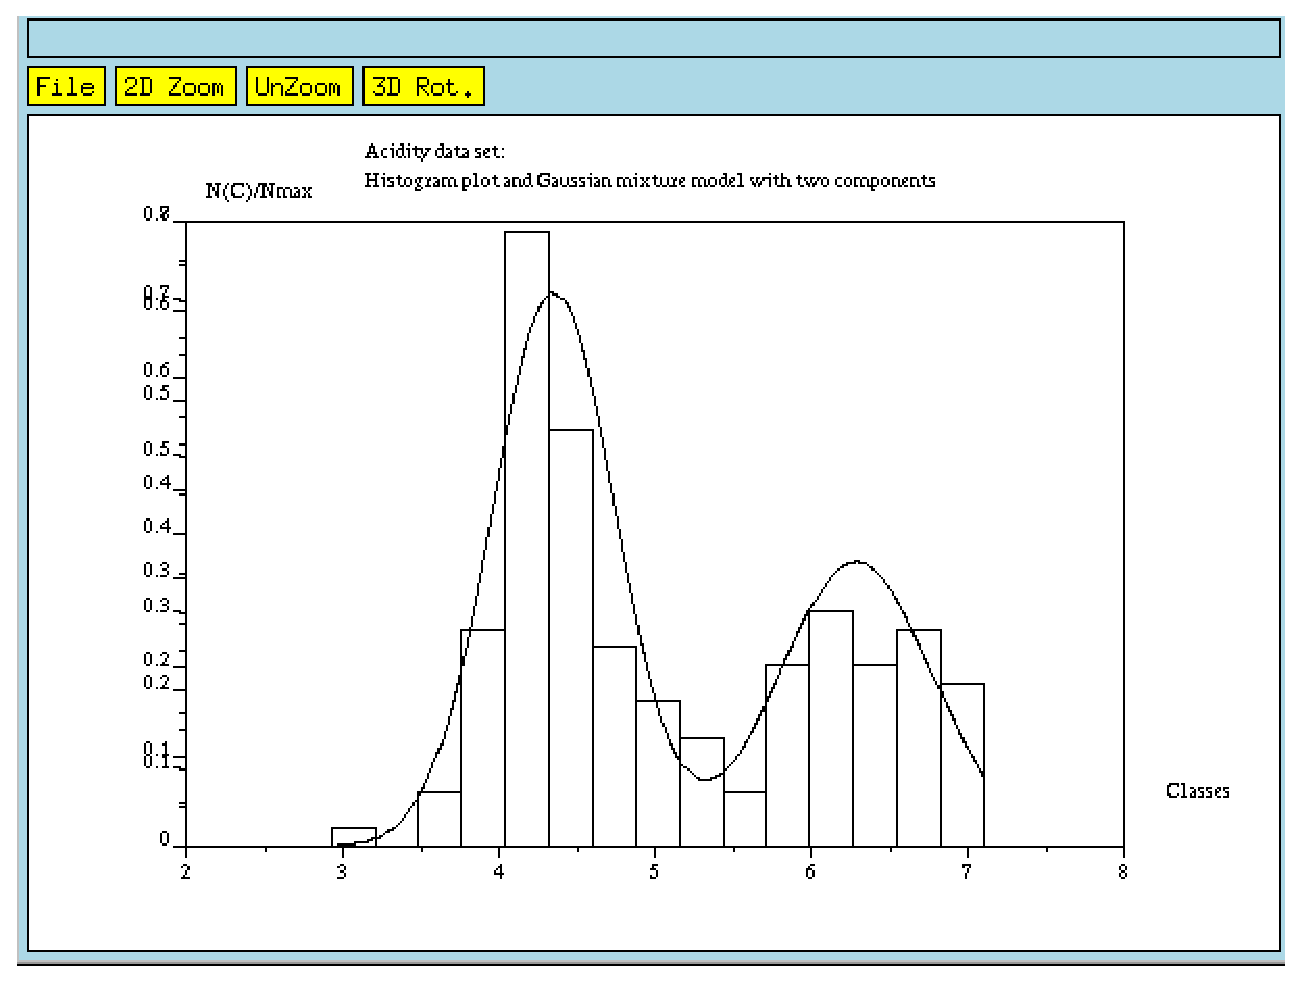
\includegraphics[width=10cm, height=7cm]{acidity.eps}
  \caption{Plot of fitted two-component normal mixture density for acidity data set.}\label{figIntro}
\end{figure}

%==============================
%==============================
\section{Areas of application }
%==============================
%==============================
The package is intended to scientists and engineers who need to
solve clustering, density estimation and classification problems. In
academic environments, it can be regarded as an instructional tool for introductory
and advanced courses in discriminant and cluster analysis. For
research scientists, an expert mode provides full capabilities for
simulations studies. In an industrial context, {\sc mixmod} is a powerful tool for research in statistical
pattern recognition.

%=======================
%=======================
\section{User interface}
%=======================
%=======================
Written in C++, {\sc mixmod} is easily interfaced with widely mathematical software Scilab and Matlab.
The {\sc mixmod} Graphical User Interface (GUI) is an important key element for
interactive statistical analysis, the user is guided step by step.
%It is the easiest way to discover {\sc mixmod} even if some particular features
%are not available in this mode. Moreover, {\sc mixmod} functions
%are available to execute {\sc mixmod} in Matlab and Scilab without using
%interface. They could be introduced in a program (see section 3.3.1 {\sc mixmod} Functions).

%=======================
%=======================
\section{Documentation}
%=======================
%=======================
The documentation around {\sc MIXMOD} is composed of a {\em User's guide}, a {\it
Statistical Manual}, a {\em Software Documentation} and a {\em Quick start Manual}.
They are available on {\sc mixmod} web site and in  {\em  $<$mixmodDir$>$/DOC} directory
and are distributed as Postscript and pdf (Acrobat Reader) files.

%===========================
%===========================
\section{Conditions of use}
%===========================
%===========================
{\sc mixmod} is publicly available under the GPL license. You can redistribute it and/or modify it under the terms of
the GPL license (www.gnu.org/copyleft/gpl.htlm).\\

Please understand that there may still be bugs and errors. Use is at your
own risk. We take no responsibility for any errors or omissions in this
package or for any misfortune that may befall you or others as a
result of its use.\\

Please report bugs at mixmod@univ-fcomte.fr

%==========================
%==========================
\section{Other softwares}
%==========================
%==========================
Several codes that are available characterize multivariate data sets as
mixtures of Gaussian populations. They include (non exhaustive list)
\begin{itemize}
   \item {\sc EMMIX} by G. McLachlan\\
    \url{http://www.maths.uq.edu.au/$\sim$gjm/emmix/emmix.html}
   \item {\sc MCLUST} by C. Fraley and A. Raftery\\
    \url{http://www.stat.washington.edu/fraley/mclust/soft.shtml}
   \item {\sc AutoClass} by P. Cheeseman\\
    \url{http://ic-www.arc.nasa.gov/ic/projects/bayes-group/autoclass/}
   \item {\sc Snob} by D. Dowe.\\
    \url{http://www.csse.monash.edu.au/$\sim$dld/Snob.html}
   \item {\sc NORMIX} by John H. Wolfe.\\
    \url{http://www.alumni.caltech.edu/$\sim$wolfe/normix.htm}
\end{itemize}
